\chapter{Model-Learning Framework}
\label{ch:methodology} %TODO Update chapter title? e.g., The Model-Learning Framework

Our interest in this thesis lies in the development of probabilistic models for systems whose dynamics are stochastic.
The objective is to use a dataset of execution traces of a system to attain an accurate system representation, which can be used to obtain plans for optimal automated control of the system under consideration.
In this chapter we describe our proposed framework that applies learning algorithms to obtain probabilistic models in the form of \acrshortpl{acr:mdp} and optimizes for a performance-maximizing model by sampling multiple hyper-parameter settings for these learning algorithms.

In \autoref{sec:model-learning-routine} a detailed explanation is provided of the learning and optimization routine which forms the basis of our framework.
Then in \autoref{sec:cost-effective-optimization} the framework is extended such that it consists of three cost-incremental phases.
Finally, in \autoref{sec:application-mobile-robot} a possible application (i.e., mobile robot navigation) of the framework is discussed, which is also used for evaluating the approach through the experiments that have been carried out and which are described in \autoref{ch:experimental-results}.

\section{Model Learning and Optimization Routine}
\label{sec:model-learning-routine}

As the development of probabilistic models oft to be a difficult an time-costly process for a human designer, an appealing idea is to automate the model development process by applying learning algorithms on a dataset of execution traces of the system under consideration.
However, to achieve effective planning in a real-world environment, the models that are learned should accurately reflect the dynamics of the system.

There are two major reasons for a learned model to not yield good performance.
First of all, the learned model may be too complicated for the amount of available data, which leads to model over-fitting.
On the other hand, one could acquire a model that is too simple to explain the available data and so does not accurately reflect the underlying system in that situation.
Therefore, the parameters of the learning algorithm should be properly adjusted in order to obtain accurate probabilistic models.

The learning and optimization routine described in this section, depicted in \autoref{fig:learning-routine-complete}, aims to achieve this by posing the adjustment of these parameters as an optimization task, with the objective of obtaining an \acrshort{acr:mdp} model that maximizes the performance of executing the plans that are derived from it.

\begin{figure}[t]
	\centering
	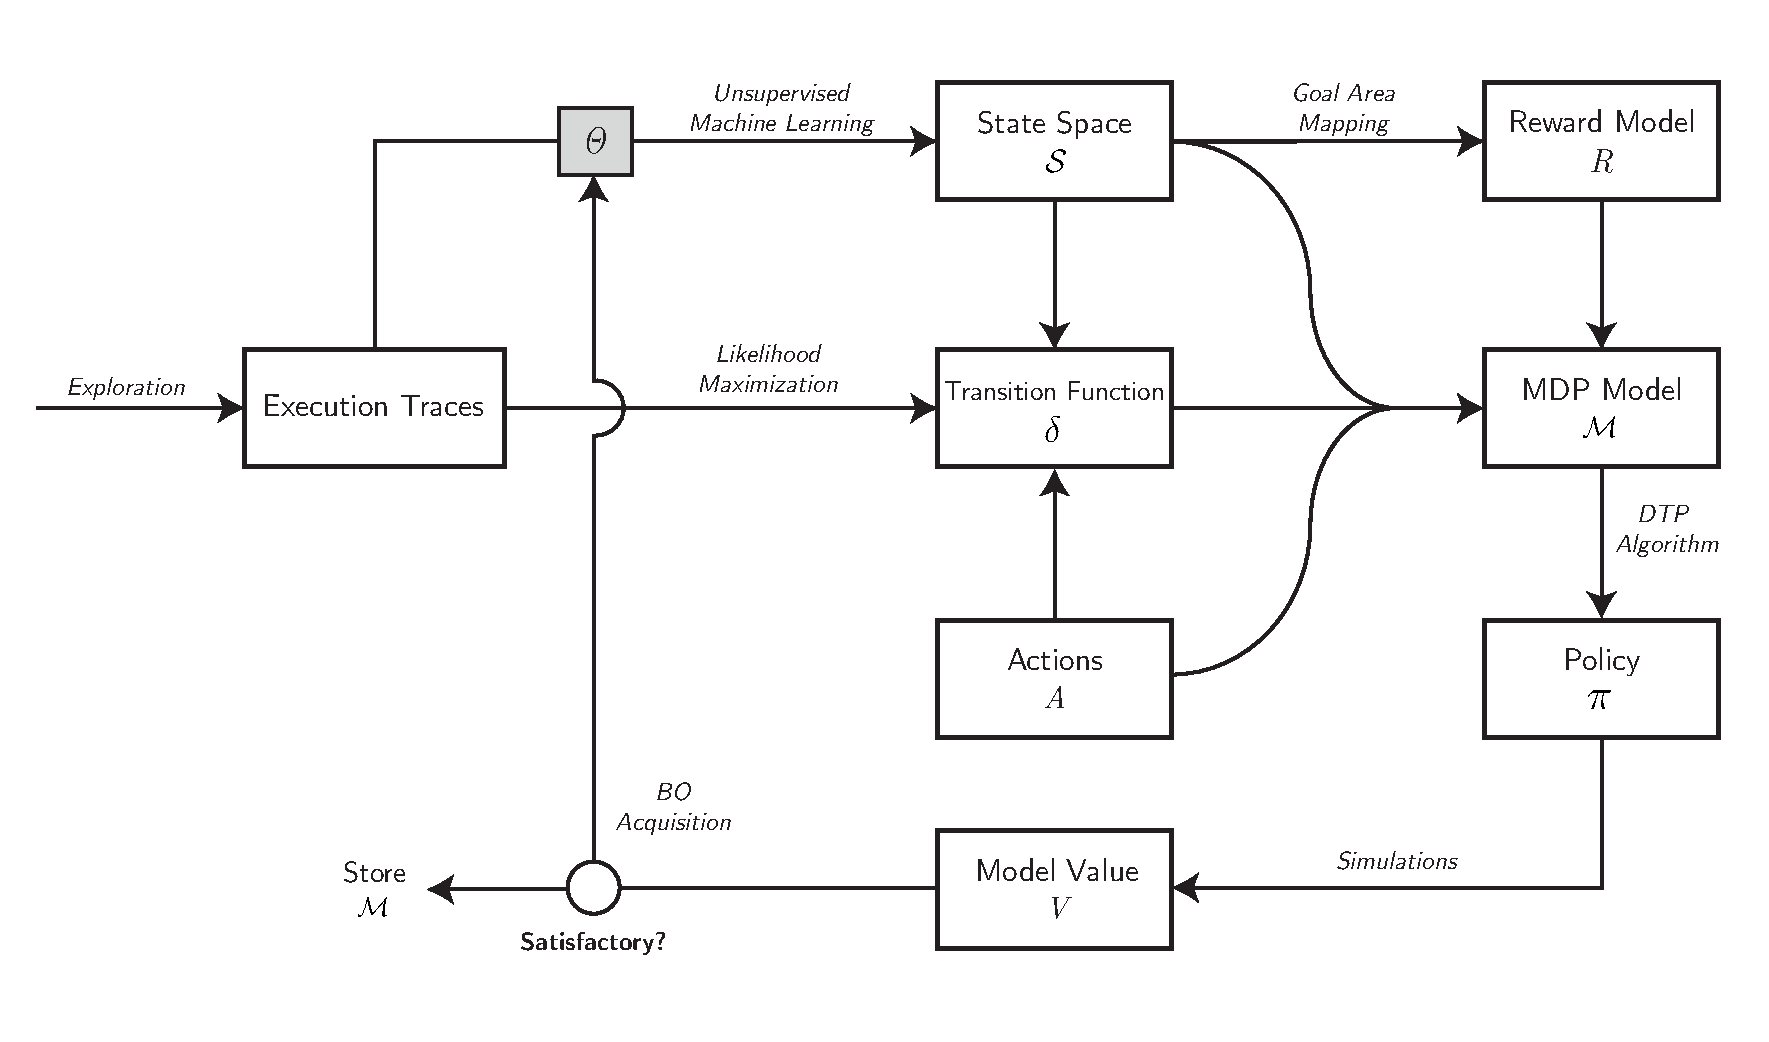
\includegraphics[width=\textwidth]{learning-cycle-complete-v2}
	\caption{Diagram of the model learning and optimization routine.}
	\label{fig:learning-routine-complete}
\end{figure}

\subsection{Learning Step}
\label{sec:routine-description}

The routine can be viewed as consisting of two subsequent steps which are repeated until an \acrshort{acr:mdp} model that yields satisfactory performance is obtained.
The first of these two main steps will be referred to as the \textit{learning step}, in which an \acrshort{acr:mdp} model is acquired.
This learning step starts off with a data-set of execution traces obtained beforehand.
Given a parameter-setting $\theta$ for a selected unsupervised machine learning algorithm, a state-space $\mathcal{S}$ is acquired using the execution traces as training set.
Subsequently a transition function $\delta$ is acquired by applying a known model-learning (as described in \autoref{sec:learning-probabilistic-models}) given the data-set, state-space $\mathcal{S}$ and possible actions $A$.
The goals of the system are accordingly mapped to a reward function $R$ over the acquired state-space $\mathcal{S}$ (or alternatively over state-action pairs or state-action-state triplets).
The state-space $\mathcal{S}$, transition function $\delta$, action set $A$, reward function $R$ and a configurable initial state $s_0$ are then combined into an \acrshort{acr:mdp} $\mathcal{M} = (\mathcal{S}, s_0, A, \delta, R)$.

To assess the performance yielded by $\mathcal{M}$, the \acrshort{acr:mdp} is solved by applying known \acrshort{acr:dtp} algorithms like \acrshort{acr:vi} or \acrshort{acr:pi} to obtain policies for a set of tasks the system is expected to perform.
The value of the model $V_{\mathcal{M}}$ is then determined by checking how well the system is expected to perform by execution according to the derived policies (e.g., based on simulations and/or the value function obtained by a \acrshort{acr:dtp} algorithm).
\autoref{sec:performance-measure} describes in detail how the performance yielded by the learned \acrshortpl{acr:mdp} is assessed and how a fair comparison of different \acrshortpl{acr:mdp} may be achieved for this routine.

%\begin{itemize}
%	\item Start off with data-set of execution traces obtained beforehand
%	\item A number of parameter-settings $\theta$ for the model-learning are initially sampled at random from a designer-specified domain $\Theta$ (i.e., the parameter-space).
%	\item Acquire state-space by an unsupervised machine learning method
%	\item Acquire transition function by applying a known model-learning algorithm as in \autoref{sec:learning-probabilistic-models} (e.g., a maximum likelihood approach)
%	\item Goals are mapped to a reward function $R$ over the acquired state-space $\mathcal{S}$ (or possibly over state-action pairs or state-action-state triplets)
%	\item Then the state-space $\mathcal{S}$, transition function $\delta$, action set $A$, reward function $R$ and a configurable initial state $s_0$ form an \acrshort{acr:mdp} $\mathcal{M} = (\mathcal{S}, s_0, A, \delta, R)$.
%	\item To asses the associated performance or value of $\mathcal{M}$, we solve the \acrshort{acr:mdp} using known \acrshort{acr:dtp} algorithms like \acrshort{acr:vi} (see \autoref{sec:planning}) to obtain one or more policies $\pi$.
%	\item The value of the model $V_\mathcal{M}$ is then determined by checking how the system would perform by execution according to the derived policies (e.g., based on simulations and/or the value function of \acrshort{acr:vi}).
%\end{itemize}

\subsection{Optimization Step}
\label{sec:optimization-step}

The second main step of the routine will be referred to as the \textit{optimization step}, in which a parameter-setting $\theta$ is selected for the next learning step in such way that yielded performance converges to a global maximum as quickly as possible.
As initially there is no knowledge of the performance given the settings of the learning parameter(s) $\theta$, in the first few routine-iterations parameter-settings are selected at random from the designer-specified domain $\Theta$ (i.e., the parameter-space).
Together with the value $V_{\mathcal{M}}$ of the corresponding model obtained in the learning step for each of these parameters $\theta$, they are stored in an evidence set $\mathcal{D}$.
The objective function $f: \Theta \mapsto \mathbb{R}$ is then defined such that it maps parameter-settings $\theta \in \Theta$ to real-valued performance yielded by \acrshortpl{acr:mdp}.

As discussed earlier in  \autoref{sec:bayesian-optimization-problem}, the objective functions for the class of \acrshort{acr:sdm} problems tend to be expensive to evaluate as proper estimations can only be made through expensive simulations.
Therefore, Bayesian optimization emerges as an attractive method to find a global maximizer $\theta^\ast \in \Theta$ for our objective function.
After each iteration the evidence set $\mathcal{D}$ is augmented with a new observation, based on which the posterior $p(f\vert \mathcal{D})$ of the objective function $f$ is updated accordingly.
A new parameter-setting for the next learning step is then sampled, corresponding to maximal utility in the selected acquisition function.

%\begin{itemize}
%	\item As said, at first a number $n$ of parameter-settings are selected randomly, stored in evidence set $\mathcal{D}$.
%	\item For these parameter-settings we obtain an estimation of the performance of executing plans derived from the learned \acrshortpl{acr:mdp}
%	\item Define the objective function $f$ such that it maps parameter-settings $\theta$ to real-valued model performance $f: \Theta \mapsto \mathbb{R}$ 
%	\item Bayesian Optimization: Motivate the application of this method to these type of problems `again'. Defines prior over $f$ and posterior based on the gathered evidence in $\mathcal{D}$.
%	\item New evidence is then acquired based on the utility function used in the optimization.
%\end{itemize}

\subsection{Performance Measure}
\label{sec:performance-measure}

\begin{figure}[t!]
\centering
\begin{tikzpicture}[->,>=stealth',auto,node distance=2.5cm,every label/.style=draw,every initial by arrow/.style={dashed}]
\tikzstyle{every state}=[fill=white,draw=black,text=black,scale=1]	% thick
\node[state,initial,initial text={},label={50:\small$+0$}] (s1) {};
\node[state,initial,initial text={},label={50:\small$+0$}] (s2) [below of=s1] {};
\node[state,initial,initial text={},label={50:\small$+0$}] (s3) [right of=s1] {};
\node[state,label={50:\small$+1$}] (goal) [below of=s3] {G};
\node[state,label={50:\small$+0$}] (trap) [right of=goal] {\text{T}};
\coordinate (con) at (0,2);
\path
(s1)
edge node {$a_i$} (goal)
(s2)
edge node {$a_j$} (goal)
(s3)
edge node {$a_k$} (goal)
(goal)
edge node {$A$} (trap)
(trap)
edge [loop above] node {$A$} (trap)
;
%\draw [->, dashed, shorten >=0pt] (s3) to[right] node[auto] {} ++(1.3,0)
;
\end{tikzpicture}
\caption{One-time reward in goal state G in an \acrshort{acr:mdp} realized by a trap state T.}
\label{fig:goal-trap-state}
\end{figure}

Posing the learning of probabilistic models as an optimization task requires us to define a mapping of \acrshortpl{acr:mdp} to a performance measure that can fairly compare different models.
As discussed earlier, one can express the performance of an \acrshort{acr:mdp} in terms of how well the agent performs tasks following policies that are derived from the model.
Therefore, one option is to make use of the value function $V$ obtained by a \acrshort{acr:dtp} algorithm (e.g., \acrshort{acr:vi} or \acrshort{acr:pi}).

One problem that emerges, however, is that there might not be a one-to-one correspondence between learned and true (goal) states, which leads to the possibility of small state spaces yielding high value while the goal states might not map well to the true goal states.
To take care of this, we introduce a discrepancy factor $\xi \in [0, 1]$, which corresponds to the fraction of data points within the goal state that map to the true goal.

Accordingly, a possible expression of how well the agent executes its task then is:
\begin{equation}
\label{eq:vdtp}
V_{\mathit{DTP},(s_0,R)} = \xi \cdot V[s_0]
\end{equation}
where $s_0 \in \mathcal{S}$ is the initial state and $R$ the reward function of the \acrshort{acr:mdp} for the task.

However, although the \acrshort{acr:dtp} algorithm may yield high value for the task, it might be that the agent will not perform well following the policy in the real world.
To better assess the performance, one could execute simulations in which the agent follows the policy derived from the \acrshort{acr:mdp} model.
Although performing simulations is more cost-expensive, it yields a better approximation of how well the agent executes a task following a policy obtained from the model.
Accordingly, let us express the performance on a task in the simulations as:
\begin{equation}
\label{eq:vsim}
V_{\mathit{SIM}, (s_0, R)} = \gamma^{t} \cdot R[i]
\end{equation}
where $s_0 \in \mathcal{S}$ is the initial state, $R$ the reward function, $\gamma$ the discount factor, $i \in \mathcal{S}$ the goal state and $t$ the number of steps taken to reach the goal.

Combining the expressions of \autoref{eq:vdtp} and \autoref{eq:vsim} yields the following expression of the performance on a task:
\begin{equation}
\label{eq:vcom}
\beta \cdot V_{\mathit{DTP}, t=(s_0, R)} + (1 - \beta) \cdot V_{\mathit{SIM}, t=(s_0, R)}
\end{equation}
where $\beta \in [0, 1]$ is a parameter which specifies the relative weight of $V_{\mathit{DTP}, t}$ against that of $V_{\mathit{SIM}, t}$ and where $s_0$ and $R$ are the initial state and reward function for the task respectively.

As the desire is to obtain a well-generalizing model that performs well on different tasks, we estimate the performance by obtaining the value yielded for multiple tasks.
To achieve this, let us first define multiple starting configurations and multiple goals for the system.
The starting configurations are each mapped to corresponding states in the \acrshort{acr:mdp}, so that one can define $\mathcal{S}_0 \subseteq \mathcal{S}$ as a set of initial states.
Similarly, the goals are each mapped to states, such that one can define $\mathcal{S}_G \subseteq \mathcal{S}$ as a set of goals.
Let us then define $R_G$ as a set of reward functions $R_i$ for each $i \in \mathcal{S}_G$ in which a one-time reward (which is realized as depicted in \autoref{fig:goal-trap-state}) is received only in goal-state $i$.
The reason the reward can only be obtained once is because in that case $V_{\mathit{DTP}, t}$ and $V_{\mathit{SIM}, t}$ will be in the same range.
Then accordingly we can define $T = \mathcal{S_0} \times R_G$ as the set of tasks, in the form of all pairs of initial and goal states, over which the performance is assessed.

\noindent Putting this all together, the performance of an \acrshort{acr:mdp} $\mathcal{M}$ can in this way be expressed as:
\begin{equation}
\label{eq:vm}
	V_{\mathcal{M}} = \frac{\sum_{\forall t \in T} \beta \cdot V_{\mathit{DTP}, t} + (1 - \beta) \cdot V_{\mathit{SIM}, t}}{|T|}
\end{equation}
where $T$ is the set consisting of the pairs of initial states and reward functions of the tasks over which the performance is assessed.

% There have been debates about the performance
% measure that should be maximized during learning {
% one point of view is that the available data should be
% used to learn all possible perceptual distinctions in the
% real world while the opposite view
% would have it that only those distinctions that are utile in actual planning and control should
% be learned [McC92]. Those algorithms that learn only utile distinctions use either decision trees
% or instance-based learning to form state representations.

%The value of \acrshort{acr:mdp} $\mathcal{M}$ is defined as:
%\begin{equation}
%	V_{\mathcal{M}} = \beta \cdot V_\mathit{DTP} + (1 - \beta) \cdot V_\mathit{SIM}
%\end{equation}
%where $\beta \in [0, 1]$ is a parameter which specifies the relative weight of $V_\mathit{DTP}$ against that of $V_\mathit{SIM}$.
%
%\begin{itemize}
%	\item Multiple starting positions/initial states
%	\item Multiple goals/reward functions
%	\item $V_\mathit{DTP}$, how to deal with problem of less states -> less steps. Need fair comparison.
%	\item Discrepancy factor; obtained value based on part of the state covering the goal
%	\item Goal state to trap state to avoid acquiring unlimited reward
%\end{itemize}

% One of the main issues faced in learning \acrshort{acr:mdp} models is that of deciding on the state space, while one typically does not know the size of the true state space of the real-world process that generated the training data.
%In fact this state space might even have been continuous, while the state space of the model is typically discrete.
%In particular this might form an issue in the planning phase where a reward function needs to be defined to express the goals in the \acrshort{acr:mdp}, for which there may not be a clear one-to-one mapping from real-world states to model states.

% Two approaches:
% - Clustering training data to obtain states
% - Trajectory Clustering

\section{Cost-Incremental Optimization}
\label{sec:cost-effective-optimization}

\begin{figure}[t]
	\centering
	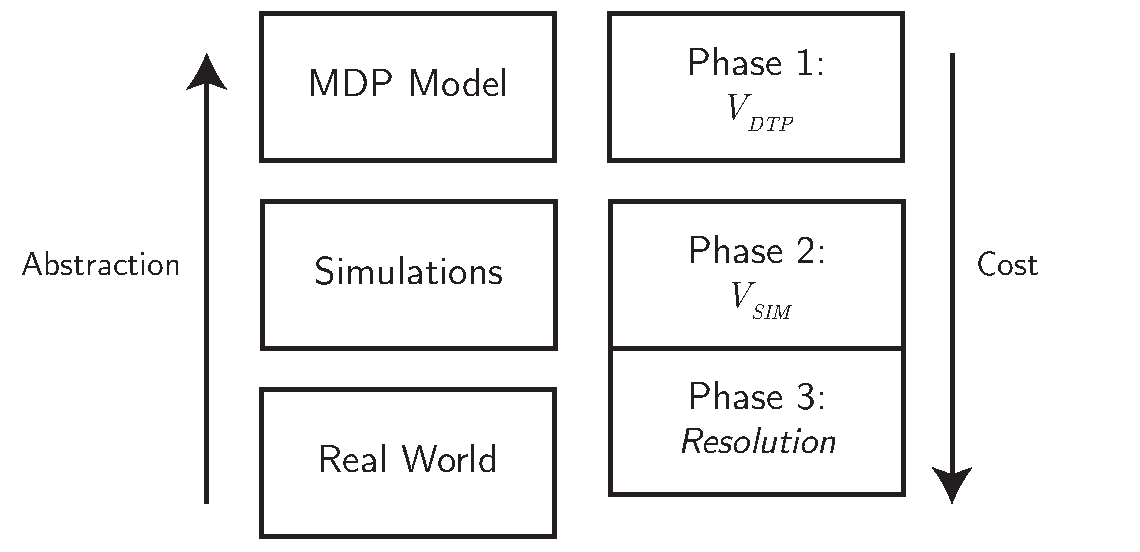
\includegraphics[width=0.7\textwidth]{abstraction-5-1}
	\caption{Correspondence of the phases of the model learning framework to the different levels of abstraction.}
	\label{fig:abstraction-cost}
\end{figure}

To make the solution more cost-effective, the framework is extended by defining three phases with the aim of exploiting the lower cost of computing the value function for \acrshortpl{acr:mdp} in comparison to the cost of executing plans in simulations or the real world.
That is, assessing performance solely based on learned \acrshort{acr:mdp} models is less cost-expensive, although the model might not accurately reflect the real world as its abstracts over low-level details.
This section defines the phases of the extension, of which each subsequent phase better reflects the real world, but on the other hand are accompanied by higher costs as is depicted in \autoref{fig:abstraction-cost}.

%\blindtext

%\begin{itemize}
%	\item Change the $\beta$-parameter of Eq 5.1 over time
%	\item The $\gamma$ discount factor (low values $\to$ faster planning)
%	\item Three 'phases':
%\end{itemize}

\subsection{Phase 1: Value Function Pre-Processing}
\label{sec:phase-1}

In the first phase the performance is assessed solely based on the value functions derived by the \acrshort{acr:dtp} algorithm used for planning.
This means the $\beta$ parameter is set to $\beta = 1$ such that the performance $V_{\mathcal{M}}$ of \acrshort{acr:mdp} $\mathcal{M}$ is expressed only in terms of $V_\mathit{DTP}$ and so no simulations are performed in this phase.
Therefore, this first phase is relatively cost-cheap, and although it abstracts from the real-world the most, it may be used to identify the interesting area of the parameter space.
Hence, the goal of this first phase is to narrow down the search space to a subspace of learning parameters more likely to yield high performance.
In practice this could be done by setting a threshold, say, $\eta \in [0, 1]$, that specifies the allowed deviation from the observed maximum in the evidence set $\mathcal{D}$, i.e. $\max_\mathcal{(x_i, y_i) \in D} y_i$, which can be used to define parameter bounds based on the posterior mean.

%First phase: Performance assessment solely based on $V_\mathit{DTP}$ (i.e., initially $\beta = 1$). No simulations. $\gamma$ parameter starts off low and increases over time. This means this first phase is relatively cost-cheap, but might give us a global idea of the interesting area of the parameter-space so that we could narrow this space down.

%\blindtext

\subsection{Phase 2: Simulation-Based Optimization}
\label{sec:phase-2}

The second phase limits the optimization to the narrowed down parameter space that follows from the first phase.
In this phase the performance assessment becomes more cost-expensive, but is also made more accurate by performing simulations and weighing the observed $V_\mathit{SIM}$ in the performance measure.
This means, we either fix the $\beta$ parameter to a value in $[0, 1)$, or alternatively, gradually decrease it over time so that $V_\mathit{SIM}$ plays a more significant role the more iterations have passed.

%Second phase: $\beta$ decreases over time, which means $V_\mathit{SIM}$ starts to play a role, and assessment becomes more accurate, but also more cost-expensive.

%\blindtext

\newpage

\subsection{Phase 3: Resolution Post-Processing}
\label{sec:phase-3}

The last phase starts when the parameter space has been narrowed down sufficiently or the parameter search has converged to an optimum.
In this phase, the goal is to further improve learned models by checking whether the transition probabilities are likely to match reality.
The identification of discrepancies in these probabilities happens by executing actions in those areas of the state-space that are visited most often and in which the agent tends to get stuck (according to the transition probabilities) and seeing if the observed transitions yield comparable probabilities.
For those areas and their corresponding states for which mismatches are identified, higher resolution is provided to better reflect the system's dynamics in the real world.
\fbox{\textbf{TODO:} Enough detail for this section?}

%Third phase: Starts when the parameter-space has sufficiently been narrowed down. To further improve learned models we would like to see if the opportunity exists of having higher resolution in some areas of the state space to better reflect the data-set.

%\blindtext

\section{Application to Mobile Robot Navigation}
\label{sec:application-mobile-robot}

\begin{figure}[t]
\centering

\captionsetup{font=small}
\captionsetup[subfigure]{font=footnotesize}
\captionsetup[subfigure]{justification=centering}
\begin{subfigure}{.5\textwidth}
	\centering
	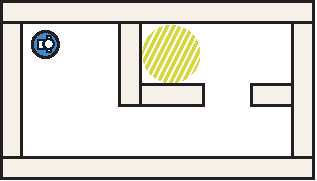
\includegraphics[width=.8\linewidth]{dummy-map-2-1}
	\caption{Dummy environment with a mobile robot and goal area.}
	\label{fig:dummy-map-1}
\end{subfigure}\hfill
\begin{subfigure}{.5\textwidth}
	\centering
	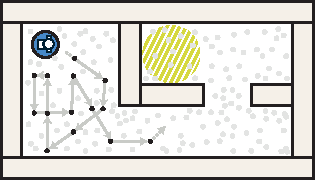
\includegraphics[width=.8\linewidth]{dummy-map-2-2}
	\caption{Data-points of execution traces from exploration depicted.}
	\label{fig:dummy-map-2}
\end{subfigure}

\bigskip

\begin{subfigure}{.5\textwidth}
	\centering
	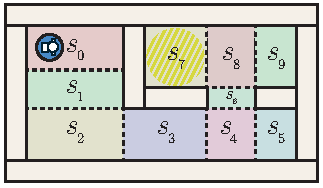
\includegraphics[width=.8\linewidth]{dummy-map-2-3}
	\caption{State-space of a learned \acrshort{acr:mdp} depicted.}
	\label{fig:dummy-map-3}
\end{subfigure}\hfill
\begin{subfigure}{.5\textwidth}
	\centering
	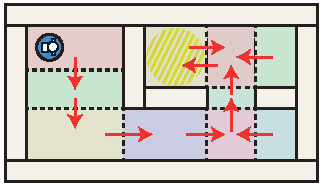
\includegraphics[width=.8\linewidth]{dummy-map-2-4}
	\caption{Corresponding optimal policy for the \acrshort{acr:mdp}.}
	\label{fig:dummy-map-4}
\end{subfigure}
	\caption{Planning for the navigation of a mobile robot by learning \acrshortpl{acr:mdp} from data about the environment.}
\end{figure}

%\begin{itemize}
%	\item Description
%	\item Motivation of this application
%	\item Generalization to other applications
%	\item Details on how we apply the framework to this application
%\end{itemize}

An example application for which the model learning framework described in this chapter could be used is that of mobile robot navigation.
The problem statement is that an agent has control over a mobile robot that should be able to navigate from one location to another in an open world, say, an office environment, as fast as possible.
This problem domain is particularly suited as the robots oft to operate under significant uncertainty in their actions (e.g., slipping) and observations (e.g., sensor noise).
Although there are other potential applications as we described in \autoref{ch:introduction}, this particular application can be used to illustrate the complete procedure of learning \acrshort{acr:mdp} from data and obtaining plans accordingly quite well.

For example, let us consider the scenario in which the robot needs to operate in an environment as depicted in \autoref{fig:dummy-map-1}.
Then, before our model learning framework is applied to learn \acrshortpl{acr:mdp} for the system, the data about the environment could have been obtained in the form of execution traces that consist of logs of the robot's location and the (next) action it's about to take.
This could then give a set of data-points, as depicted in \autoref{fig:dummy-map-2}, which can be used to learn the states and transition probabilities of an \acrshort{acr:mdp}.
A potential state-space of an \acrshort{acr:mdp} that might be learned from this dataset is shown in \autoref{fig:dummy-map-3}.
Then, assigning a reward to a state that covers the goal area should give us a policy that leads the robot from any initial state to the goal state as depicted in \autoref{fig:dummy-map-4}.

\newpage

In this application the performance of a learned \acrshort{acr:mdp} can be assessed as described in \autoref{sec:performance-measure} through the computed value function and performing simulations for the various tasks the robot should be able to execute.
Comparing the performance that was assessed for multiple \acrshort{acr:mdp} through the framework on convergence leads to an \acrshort{acr:mdp} that reflects the real world and generalizes over multiple tasks quite well.




%% OLD %%

%\textbf{Note:} These bullet-points have not been completely updated yet although most are still relevant. Outline should be such that we first discuss the framework for model learning and optimization without considering incomplete data or doing cost-sensitive optimization, which are discussed next ('why and how').
%Probably describing the framework should be separated from the application to mobile robot navigation and how it is implemented, which should be described afterwards.
%
%\begin{itemize}
%	\item Introduction
%	\item Explain high-level algorithm idea?
%\end{itemize}
%
%\section{Application}
%\label{sec:application}
%
%% 
%
%\begin{itemize}
%	\item Mobile robot navigation
%	\item Why this application?
%	\item Generalization possible to other applications?
%\end{itemize}
%
%\section{Exploration Phase}
%\label{sec:exploration-phase}
%
%% 
%
%\begin{itemize}
%	\item Obtain a dataset of observations, for our application this concerns data about attainable positions of the robot that will be controlled
%	\item Under the assumption such a dataset is not yet available to us, this dataset is retrieved in an exploration phase
%	\item In this exploration phase, the robot should explore the environment and periodically record information about its current position while aiming to visit all the locations of importance
%	\item This exploration phase is (preferably) only carried out once
%	\item To obtain a dataset for our tests the exploration phase is carried out in a robot simulator. Should also explain what data is obtained in this exploration.
%	\item The overall algorithm is tested for multiple maps/(office-like) environments, which might differ in their dimensions, number of obstacles or `openness'.
%	\item To take into account dynamically changing environments to some extent, there are also doors that will be open or closed as time passes.
%	\item The simulations are carried out in the Morse simulator, in which the exploration is carried out by an agent that randomly navigates an environment.
%\end{itemize}
%
%\section{State Space Acquisition}
%\label{sec:state-space-aggregation}
%
%% 
%
%\begin{itemize}
%	\item Using exploration data
%	\item Unsupervised machine learning to obtain states for an MDP model (various possible methods possible: e.g., kmeans, gmm)
%	\item Unknown parameter $\delta$ of the unsupervised machine learning algorithm to be optimized
%\end{itemize}
%
%\section{Model and Policy Acquisition}
%\label{sec:model-policy-acquisition}
%
%% 
%
%\begin{itemize}
%	\item State space obtained as described in previous section
%	\item Transition function obtained based on exploration data and state space through the likelihood maximization approach.
%	\item For our application the actions are fixed and can either be \textsc{NORTH}, \textsc{EAST}, \textsc{SOUTH}, \textsc{WEST} which makes the robot navigate in the corresponding direction.
%	\item Rewards
%	\item Timesteps
%	\item Policy (various possible `solvers': value iteration, policy iteration)
%\end{itemize}
%
%\section{Bayesian Model Optimization}
%\label{sec:bayesian-model-optimization}
%
%% 
%
%\begin{itemize}
%	\item Optimization of the unknown $\delta$ parameter of the machine learning algorithm for state space aggregation
%	\item Evaluation by simulations of the found policy for the given $\delta$ parameter
%	\item ...
%\end{itemize}
%
